\noindent\textbf{General Trends}\newline

Participants were given 4 calendar weeks to code, process, and finalize a turbine placement that delivered their proposed optimal AEP.
All participants are volunteers, and their participation was conducted outside of normal work or educational responsibilities.
This 4-week optimization window factors to be $0.2\%$ of typical wind farm's 20-year lifespan \cite{HerbertAcero2014}, and we submit that optimizations (even if needing the full extent of this timeframe) would be worth the time they require, if able to produce superior results.
However, from the participant self-reported wall-times, none of the optimizations took nearly that long.

For this reason, we discounted required wall time as a distiguishing factor, and use resultant AEP as our main metric for measuring algorithm effectiveness.
Though factors like processing time and computing power do vary, we consider algorithms that produce results anywhere within the 4 week announcement-to-call window to be acceptable for applications in industry.

%The participant data is multivariate, leading to numerous inferences.
As a general trend, gradient-based methods performed better in discovering a relative optima, especially for smaller farm sizes.
Some gradient-based algorithms improved in comparative performance as the number of design variables increase (\textit{par10}, \textit{par3}), while others degrade (\textit{par5}, \textit{par8}).
Simultaneously, some gradient-free algorithms increase in effectiveness as design variables increase (\textit{par2}, \textit{par3}), while others compete for worst comparative performance, regardless of farm size (\textit{par6}, \textit{par7}, \textit{par9}).

Despite these multi-variate results, one clear front-runner does emerge.
Regardless of wind farm size, \textit{par4}'s algorithm, consistently discovered turbine placement that delivers an AEP superior to all other participants.
A summary of \textit{par4}'s method is included in a following section.

Also of note, as the number of design variables increases, the relative disparity between proposed optimal AEPs likewise diverge.
For the 16 turbine case, the best result is $7.88\%$ better than the worst.
For the 36 and 64 cases, the best result is $11.45\%$ and $13.54\%$ better than the worst, respectively.

%\subsubsection{Participant List}

\subsubsection{Analysis of Best Results}

	\vspace{3mm}
	\noindent\textbf{Gradient-based}\newline

	For all 3 farm sizes, the superior method was implemented by \textit{par4}, using a gradient-based method.
	Coded in Python and FORTRAN, it combined the Sparse Nonlinear OPTimizer (SNOPT) \cite{SNOPT} with a sampling method called Wake Expansion Continuation (WEC) \cite{Thomas2018}.
	Running 200 optimizations, \textit{par4} had one iteration start from the provided example layout, and the other 199 use randomized turbine starting locations within the farm boundary.

	The WEC method is specifically designed to reduce the multi-modality found in wind farm layout optimization.
	In the cited paper\cite{Thomas2018}, it is also referred to as a Design Space Relaxation Optimization Process (DSROP).
	DSROP is a method of converting design spaces with many local minima into curves approaching convexity, allowing gradient-based optimizations to more easily find the global solution.
	An example of such ``relaxation'' to convexity is included in \cref{fig:wec1,fig:wec2}, reproduced for description.

	\begin{figure}
		\centering
		\begin{minipage}{.43\textwidth}
		  \centering
		  \captionsetup{width=0.85\textwidth}
		  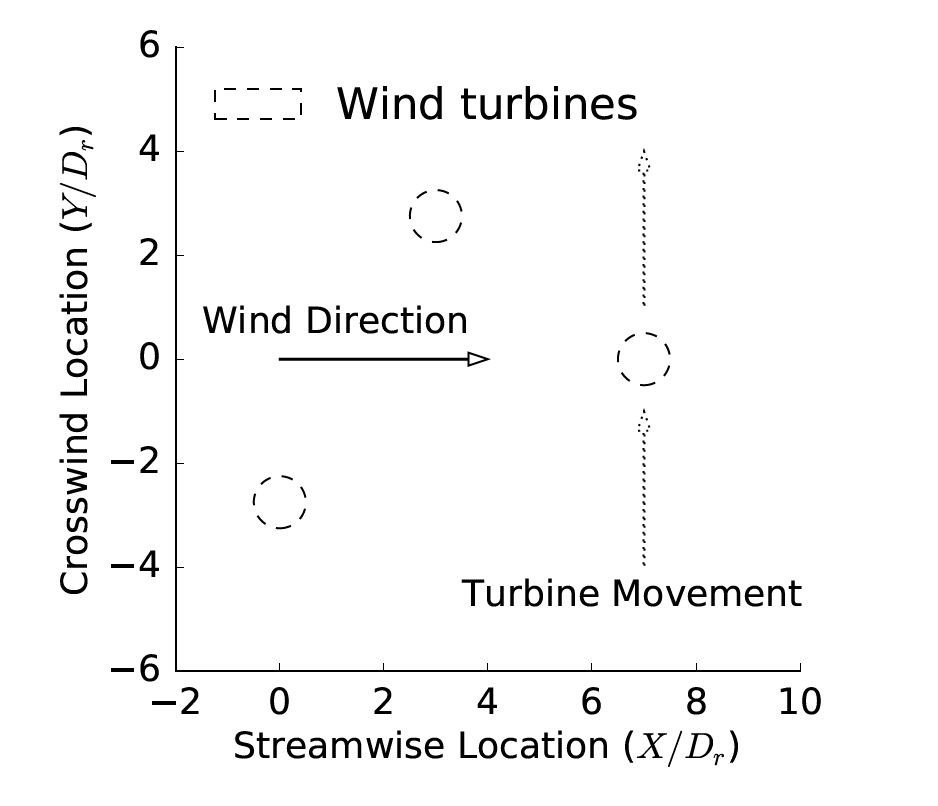
\includegraphics[width=\textwidth]{./figures/thomas-wec1.png}
		  \caption{Simple design space used to
		  	demonstrate the effects of the relaxation
			factor, $\xi$, on the wind farm layout design space. \cite{Thomas2018}}
		  \label{fig:wec1}
		\end{minipage}%
		\begin{minipage}{.5\textwidth}
		  \centering
		  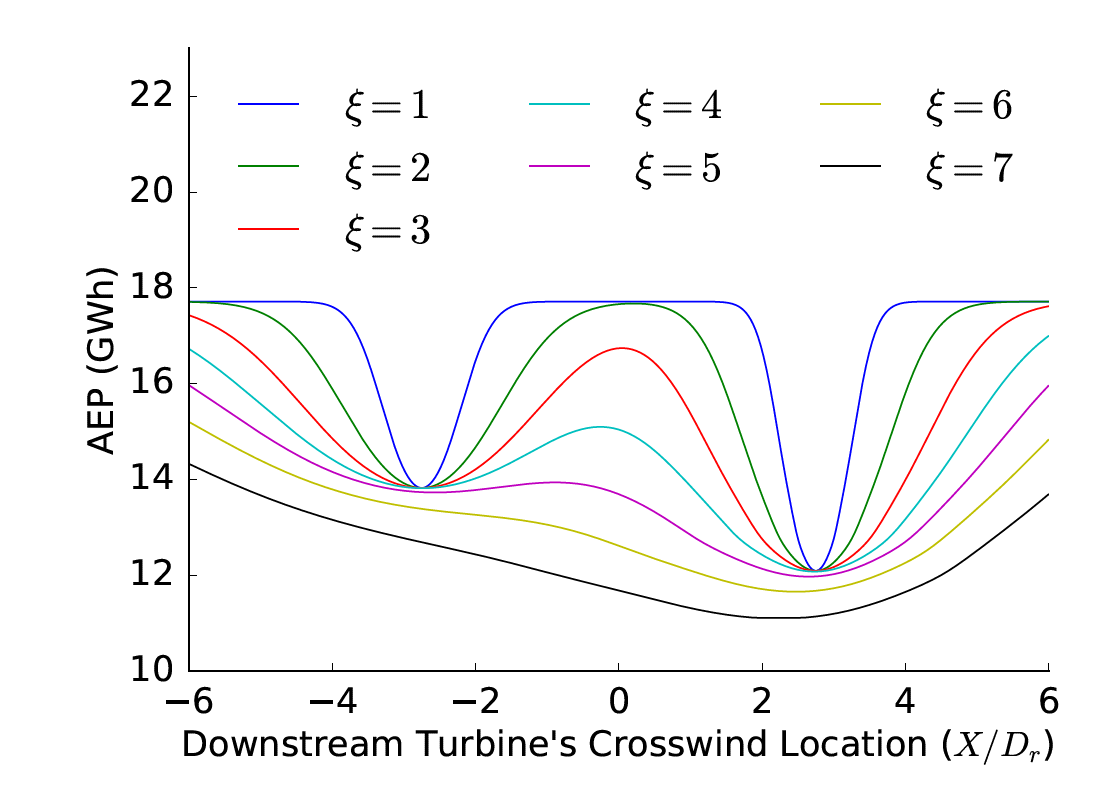
\includegraphics[width=\textwidth]{./figures/thomas-wec2.png}
		  \caption{The impact of the wake relaxation factor, $\xi$.
		  One turbine was moved across the wakes of two upstream turbines (see \cref{fig:wec1}). \cite{Thomas2018}}
		  \label{fig:wec2}
		\end{minipage}
	\end{figure}

	\cref{fig:wec1,fig:wec2} demonstrate the effects of the WEC method on a simple design space, relaxing the local optima into a more easily discovered global solution.
	As the author J.J. Thomas states, ``Larger values of $\xi$ allow the smaller local optima to disappear completely.
	Smaller values of $\xi$ allow for more accurate wake widths but with an increase in the number and magnitude of local optima.'' \cite{Thomas2018}.
	We suspect that this WEC sampling method for relaxing the multi-modality of the design space is the reason that \textit{par4}'s optimizatons found superior layouts to the other used methods.

	\vspace{3mm}
	\noindent\textbf{Gradient-free}\newline

	Of the gradient-free methods used, the superior particiant was \textit{par2}.
	Futhermore, the relative performance increased as wind farm size increased.
	Out of the 10 participants, \textit{par2} ranked 5th, 3rd, then 2nd as the turbine sizes went from 16, to 36, to 64.
	
	Programmed in Python, \textit{par2} used a ``Preconditioned'' Sequential Quadratic Programming (SQP) optimization method.
	SQP is an optimization method which breaks the problem into quadratic subproblems.
	To seed steps between generations, \textit{par2} took a starting layout and rotated it in $\pi$/6 steps.
	The best of the 12 resultant layouts was then taken as the warm-start for the next generation.

	%still don't know how he did it. pyOpt??


\subsubsection{Analysis of Worst Results}
	\vspace{3mm}
	\noindent\textbf{Gradient-based}\newline
	
	The worst performing gradient-based approach was different for each wind farm size.
	For the 16 turbine farm, \textit{par10}'s method was the poorest performing gradient-based method, but climed to the second best gradient method for the large sizes.
	For the 36 turbine farm, \textit{par1} was the poorest gradient-based method, but for the 64 turbine case, outperformed two other gradient-based methods.
	For the 36 turbine farm, \textit{par5}'s attempt was the worst gradient-based method performance, and poorer than almost all of the gradient-free methods as well.

	Not using the Python implementation we supplied, \textit{par5} translated the target AEP function into MATLAB and used that language's built-in FMINCON() function to optimize turbine locations.
	For the 16 farm case, \textit{par5} did 1000 optimizations, each with randomized turbine starting locations.
	Due to computational time required, \textit{par5} did only 500 random starts for the 64 turbine case, and this poorer relative performance may be a result of the smaller sample size.

	\vspace{3mm}
	\noindent\textbf{Gradient-free}\newline

	Two participants using gradient-free methods (\textit{par6}, \textit{par7}) rotated positions for lowest relative AEP.
	They each used a different method, and will be described individually.

	Coding in MATLAB, \textit{par6} used a multi-start partical swarm, with the interior point method.
	For each farm size \textit{par6} did 300 optimizations, with 20 swarm particles.
	If the minimum distance between turbines was violated at the end of an iteration, \textit{par6}'s algorithm randomized a new turbine location within the boundary and spacing constraints.
	The swarm algorithm used an inertia weight 0.729, and social and cognitive weights of 1.49618.
	The initial turbine location population used only turbine coordinates satisfying the boundary and spacing constraints.

	Coding in Python, \textit{par7} used a genetic algorithm.
	The algorithm used a tournament selection method, with n=10 and elitism, where only the highest AEP layouts went on to seed the next generation.
	There were 25 generations each of size 500, using a mutation probability of 3\%.

\subsubsection{Discussion}

	No worst-practices pattern can be concluded from the 3 cases, as the poorest performers all had vastly different methods for reaching their results.

	In terms of best-practices, for the 3 farm sizes we tested, \textit{par4}'s strategy of using the SNOPT optimizer combined with the WEC relaxation method consistently delivered superior layouts.

	Though \textit{par4} consistently found the superior AEP relative to the other participants, \textit{par2}'s results demonstrate a trend closing the gap as the number of design variables increased.
	For the 16 turbine case, \textit{par4} was 2.5\% better than \textit{par2}'s results.
	For the 36 and 64 cases, \textit{par4} was 1.68\% and 0.46\% better, respectively.
	It should be noted, however, that at the current average U.S. rate\cite{ChooseEnergyCost} of roughly \cent 13.3 for a kWh (or \$133 per MWh), the income difference between the AEPs of \textit{par4} and \textit{par2} in the 64 turbine case, though only 0.46\%, equates to a difference of a little under 1 million U.S. dollars.
	
	Since \textit{par2}'s SQP method steadily closed the gap, a future study should test even larger wind farm sizes.
	This could determine if the SQP algorithm will eventually outperform the SNOPT \texttt{+} WEC method when a certain number of design variables are reached, or if there is an upper limit or convergence to this trend.